\documentclass[10pt]{article}
% =====================================================================
%  The Heraclitean Representation Hypothesis
%  Build:  make paper   (pdflatex + bibtex; arXiv-compatible, no shell-escape)
%  All real-data numbers come from generated/*.tex written by `run_hrh.py eval`.
% =====================================================================
\usepackage[T1]{fontenc}
\usepackage[utf8]{inputenc}
\usepackage{amsmath, amsthm}          % amsthm must precede newtxmath (\openbox)
\usepackage{newtxtext}
\usepackage[varvw]{newtxmath}
\usepackage[letterpaper, margin=1in, headheight=14pt]{geometry}
\usepackage{microtype}
\usepackage{mathtools, bm}
\usepackage{graphicx, booktabs, tabularx, multirow, array, caption, subcaption}
\usepackage{enumitem, xcolor, tikz, float, placeins}
\usepackage[most]{tcolorbox}
\usepackage[numbers, sort&compress]{natbib}
\usepackage{fancyhdr}
\usepackage[hidelinks]{hyperref}
\usepackage{xurl}
\usepackage[capitalize, noabbrev]{cleveref}
\usetikzlibrary{arrows.meta, calc, shapes.geometric, decorations.pathmorphing}

% ------------------------------------------------------------ palette (matches figures)
\definecolor{hrhblue}{HTML}{2A78D6}
\definecolor{hrhorange}{HTML}{EB6834}
\definecolor{hrhaqua}{HTML}{1BAF7A}
\definecolor{hrhgreen}{HTML}{008300}
\definecolor{hrhviolet}{HTML}{6250D6}
\definecolor{hrhink}{HTML}{0B0B0B}
\definecolor{hrhink2}{HTML}{52514E}
\definecolor{hrhmuted}{HTML}{8A8984}
\definecolor{hrhsurface}{HTML}{F4F3F0}
\definecolor{hrhlink}{HTML}{1C5CAB}
\hypersetup{colorlinks=true, linkcolor=hrhlink, citecolor=hrhlink, urlcolor=hrhlink}

% ------------------------------------------------------------ layout
\captionsetup{font=small, labelfont=bf, labelsep=period, skip=4pt}
\setlist{itemsep=1pt, topsep=3pt, leftmargin=1.4em}
\pagestyle{fancy}\fancyhf{}
\renewcommand{\headrulewidth}{0pt}
\fancyhead[R]{\small\textcolor{hrhmuted}{The Heraclitean Representation Hypothesis}}
\fancyfoot[C]{\small\thepage}
\setlength{\parskip}{0pt}

% ------------------------------------------------------------ theorem environments
\theoremstyle{plain}
\newtheorem{theorem}{Theorem}
\newtheorem{proposition}{Proposition}
\newtheorem{corollary}{Corollary}
\newtheorem{lemma}{Lemma}
\theoremstyle{definition}
\newtheorem{definition}{Definition}
\newtheorem{hypothesis}{Hypothesis}
\theoremstyle{remark}
\newtheorem{remark}{Remark}
\crefname{hypothesis}{Hypothesis}{Hypotheses}

\newtcolorbox{claimbox}[1][]{enhanced, breakable, colback=hrhsurface, colframe=hrhsurface,
  boxrule=0pt, arc=3pt, left=8pt, right=8pt, top=6pt, bottom=6pt,
  borderline west={2.2pt}{0pt}{hrhblue}, #1}
\newtcolorbox{pendingbox}{enhanced, colback=white, colframe=hrhmuted, boxrule=0.5pt,
  arc=3pt, left=8pt, right=8pt, top=6pt, bottom=6pt, fontupper=\small\color{hrhink2}}

% ------------------------------------------------------------ notation
\newcommand{\R}{\mathbb{R}}
\newcommand{\E}{\mathbb{E}}
\newcommand{\K}{\mathcal{K}}
\newcommand{\T}{\top}
\newcommand{\fro}[1]{\left\lVert #1 \right\rVert_F}
\newcommand{\ip}[2]{\left\langle #1, #2 \right\rangle_F}
\newcommand{\row}{\operatorname{row}}
\newcommand{\CKA}{\operatorname{CKA}}
\newcommand{\Align}{\operatorname{Align}}
\newcommand{\DHRH}{D_{\mathrm{HRH}}}
\newcommand{\Cov}{\operatorname{Cov}}
\newcommand{\tbd}{\textcolor{hrhmuted}{\textsc{tbd}}}
% primitive \input: expandable, so generated table rows work inside tabular
\makeatletter\newcommand{\tabinput}[1]{\@@input #1 }\makeatother

% ------------------------------------------------------------ generated numbers
% Defaults until `run_hrh.py paper` writes generated/v2.tex (flips \hrhvtwotrue).
\newif\ifhrhvtwo \hrhvtwofalse
\newcommand{\vNdev}{33}\newcommand{\vNheld}{18}\newcommand{\vNall}{51}
\newcommand{\vLawVerdict}{\tbd}\newcommand{\vHash}{\tbd}\newcommand{\vSlopeBound}{\tbd}
\newcommand{\vdefault}[1]{\expandafter\newcommand\csname #1\endcsname{\tbd}}
\vdefault{vRhoEarly}\vdefault{vRhoMid}\vdefault{vRhoLate}
\vdefault{vParEarly}\vdefault{vParMid}\vdefault{vParLate}
\vdefault{vCvEarly}\vdefault{vCvMid}\vdefault{vCvLate}
\vdefault{vCvREarly}\vdefault{vCvRMid}\vdefault{vCvRLate}
\vdefault{vBEarly}\vdefault{vBMid}\vdefault{vBLate}
\vdefault{vNoFcEarly}\vdefault{vNoFcMid}\vdefault{vNoFcLate}
\vdefault{vVarFamEarly}\vdefault{vVarFamMid}\vdefault{vVarFamLate}
\vdefault{vVarSizeEarly}\vdefault{vVarSizeMid}\vdefault{vVarSizeLate}
\vdefault{vSlopeEarly}\vdefault{vSlopeMid}\vdefault{vSlopeLate}
\vdefault{vVarFamMin}\vdefault{vVarFamMax}
\newif\ifhrhconv \hrhconvfalse
\vdefault{vConvSlopeOut}\vdefault{vConvSlopeMid}\vdefault{vAgreeQ}\vdefault{vAgreeOut}
\vdefault{vAgreeSameTQ}\vdefault{vAgreeSameOut}\vdefault{vAgreeDiffQ}\vdefault{vAgreeDiffOut}
\vdefault{vConvBrainEarly}\vdefault{vConvBrainMid}\vdefault{vConvBrainLate}
\InputIfFileExists{generated/v2.tex}{}{}
\InputIfFileExists{generated/synthetic.tex}{}{}
\newcommand{\vjoin}[3]{#1, #2 and #3}

% =====================================================================
\title{%
  \vspace{-1.2em}
  {\LARGE\bfseries The Heraclitean Representation Hypothesis}\\[6pt]
  {\large What a network learns to predict, not its size, sets which moment of perception it matches}}
\author{%
  \textbf{Talha R\"uzgar Akku\c{s}}\\[2pt]
  {\small\texttt{talharuzgarakkus@gmail.com}}\quad
  {\small\href{https://github.com/LegallyCoder/hrh}{\texttt{github.com/LegallyCoder/hrh}}}}
\date{}

\begin{document}
\maketitle
\thispagestyle{empty}

\begin{abstract}
\noindent
The Platonic Representation Hypothesis holds that as neural networks scale, their
representations converge to a single model of reality. Biological vision, however, is not a
single representation but a trajectory: within a few hundred milliseconds, visual cortex passes
through retinotopic, semantic and recurrent regimes. We ask which part of that trajectory a
network can match, and what determines it. Across \vNall{} vision models and ten human
subjects (THINGS-EEG2), the answer is not scale. Within six scaling ladders spanning 6M to
1.8B parameters, alignment is flat in model size in every time window, with every 95\% interval
excluding slopes larger than \vSlopeBound{} per decade, while model family accounts for
\vVarFamMin--\vVarFamMax\% of the variance between models. Between models, agreement is highest in
early layers and falls with depth, while networks that share an objective re-converge at the
readout. We explain these results with a theory of \emph{spectral trajectories}: in deep linear networks trained on natural-image statistics, the
layers of a network pass through a sequence of representational spectra that runs from the
input's to an endpoint fixed by the objective; width does not enter, and depth only refines the
steps. Alignment with a processing stage peaks where the spectra match. Turning the theory into
a law, we predict each model's alignment from properties measured \emph{without any neural
data}, fit the law on \vNdev{} development models, register its predictions for \vNheld{}
held-out models from seven objectives, and only then compute their alignment. The registered
test is \textbf{\vLawVerdict}: the law ranks held-out models with Spearman
$\rho$ = \vRhoEarly{} (early), \vRhoMid{} (semantic) and \vRhoLate{} (late), where model size
ranks them at chance.
\end{abstract}

% =====================================================================
\begin{figure}[t]
  \centering
  % Figure 1 — Platonic vs. Heraclitean picture of representational convergence.
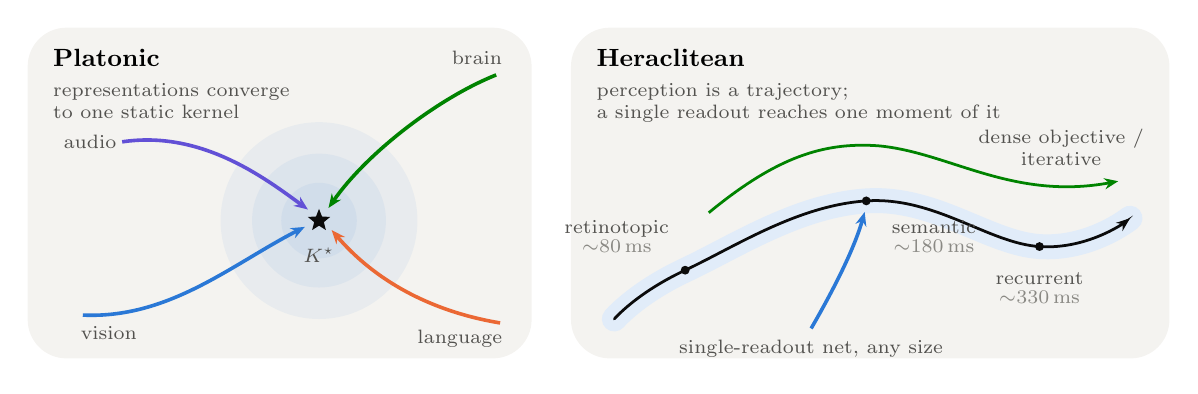
\begin{tikzpicture}[
    x=1cm, y=1cm, font=\footnotesize,
    lab/.style={text=hrhink2, font=\scriptsize, align=center},
    model/.style={line width=1.3pt, -{Stealth[length=5pt,width=4pt]}},
  ]
  % ------------------------------------------------------------ left: PRH
  \begin{scope}
    \fill[hrhsurface, rounded corners=14pt] (0,0) rectangle (6.4,4.2);
    \node[anchor=north west, font=\small\bfseries] at (0.2,4.05) {Platonic};
    \node[anchor=north west, lab, align=left] at (0.2,3.62) {representations converge\\to one static kernel};
    \coordinate (K) at (3.7,1.75);
    \foreach \r/\o in {1.25/18, 0.85/30, 0.48/45}{
      \fill[hrhblue, opacity=0.06] (K) circle (\r);
    }
    \draw[model, hrhblue]   (0.7,0.55) .. controls (1.8,0.5) and (2.6,1.2) .. ($(K)+(-0.18,-0.08)$);
    \draw[model, hrhorange] (6.0,0.45) .. controls (5.1,0.6) and (4.4,1.0) .. ($(K)+(0.16,-0.12)$);
    \draw[model, hrhgreen]  (5.95,3.6) .. controls (5.2,3.3) and (4.3,2.6) .. ($(K)+(0.12,0.16)$);
    \draw[model, hrhviolet] (1.2,2.75) .. controls (2.2,2.9) and (3.0,2.3) .. ($(K)+(-0.14,0.14)$);
    \node[star, star points=5, star point ratio=2.3, fill=hrhink, inner sep=1.3pt] at (K) {};
    \node[lab, anchor=north] at ($(K)+(0,-0.22)$) {$K^{\star}$};
    \node[lab, anchor=west] at (0.55,0.32) {vision};
    \node[lab, anchor=east] at (6.15,0.25) {language};
    \node[lab, anchor=east] at (6.15,3.82) {brain};
    \node[lab, anchor=east] at (1.25,2.75) {audio};
  \end{scope}
  % ------------------------------------------------------------ right: HRH
  \begin{scope}[xshift=6.9cm]
    \fill[hrhsurface, rounded corners=14pt] (0,0) rectangle (7.6,4.2);
    \node[anchor=north west, font=\small\bfseries] at (0.2,4.05) {Heraclitean};
    \node[anchor=north west, lab, align=left] at (0.2,3.62) {perception is a trajectory;\\a single readout reaches one moment of it};
    % the river: brain trajectory over time (regime points lie on the curve)
    \coordinate (S0) at (0.55,0.5); \coordinate (E) at (1.45,1.12);
    \coordinate (M) at (3.75,2.0);  \coordinate (L) at (5.95,1.42); \coordinate (S1) at (7.1,1.78);
    \draw[line width=9pt, hrhblue!14, line cap=round] plot[smooth, tension=0.7] coordinates {(S0) (E) (M) (L) (S1)};
    \draw[line width=1.0pt, hrhink, line cap=round, -{Stealth[length=5pt]}]
        plot[smooth, tension=0.7] coordinates {(S0) (E) (M) (L) (S1)};
    \fill[hrhink] (E) circle (1.6pt) (M) circle (1.6pt) (L) circle (1.6pt);
    \node[lab, anchor=south east] at ($(E)+(-0.08,0.1)$) {retinotopic\\[-1pt]\textcolor{hrhmuted}{$\sim$80\,ms}};
    \node[lab, anchor=north west] at ($(M)+(0.2,-0.12)$) {semantic\\[-1pt]\textcolor{hrhmuted}{$\sim$180\,ms}};
    \node[lab, anchor=north] at ($(L)+(0,-0.2)$) {recurrent\\[-1pt]\textcolor{hrhmuted}{$\sim$330\,ms}};
    % single-readout net (any size): jumps straight to the semantic point
    \draw[model, hrhblue] (3.05,0.38) .. controls (3.35,0.9) and (3.6,1.4) .. ($(M)+(-0.02,-0.14)$);
    \node[lab, anchor=north] at (3.05,0.36) {single-readout net, any size};
    % iterative / multi-readout model: tracks the whole river
    \draw[model, hrhgreen, line width=1.0pt] (1.75,1.85) .. controls (2.6,2.55) and (3.2,2.75) .. (3.9,2.7)
        .. controls (4.8,2.62) and (5.6,2.0) .. (6.95,2.25);
    \node[lab, anchor=south east] at (7.4,2.33) {dense objective /\\iterative};
  \end{scope}
\end{tikzpicture}

  \caption{\textbf{Two pictures of convergence.} \emph{Left:} the Platonic picture, in which
    systems converge on one static similarity kernel $K^\star$. \emph{Right:} the Heraclitean
    picture. Perception is a trajectory through representational regimes. A network trained
    through a single readout reaches the semantic point whatever its size; which other parts of
    the path it can match is set by what it is trained to predict.}
  \label{fig:teaser}
\end{figure}

\section{Introduction}
\label{sec:intro}

\begin{quote}\small\itshape
  ``You could not step twice into the same river.''\hfill
  \textup{--- Heraclitus, as reported by Plato, \emph{Cratylus} 402a~\citep{plato_cratylus}}
\end{quote}

\noindent
\citet{huh2024platonic} observe that independently trained models come to agree on which inputs
are similar, and that agreement grows with scale. They read this as convergence toward a shared
statistical model of reality. If that reading is right, scale is a road to brain-like
representations, and alignment with biological vision should grow with capability.

A representation in this sense is one similarity kernel read out at one layer. Visual cortex,
however, computes a sequence of kernels: low-level, retinotopic structure from about 50\,ms,
object and category structure from about 120\,ms, and later recurrent, context-dependent
processing~\citep{cichy2016comparison,kietzmann2019recurrence,kar2019recurrent}. Comparing a
network with the brain therefore means asking \emph{which moment} of this process it matches.
We call the view that convergence must be assessed over such trajectories the
\textbf{Heraclitean Representation Hypothesis} (HRH), after the philosopher of flux whom Plato's
theory of Forms was built to answer.

\paragraph{Contributions.}
\begin{enumerate}
  \item \textbf{Scale does not move alignment} (\cref{sec:scale}). Across six scaling ladders,
    alignment with every window of the EEG time course is flat in size. The same pipeline
    detects differences between objectives several times larger, so the null is not a matter
    of sensitivity.
  \item \textbf{A theory of spectral trajectories} (\cref{sec:theory}). Under natural-image
    statistics, the layers of a trained deep linear network trace a fixed path through
    representational spectra, from the input's to an objective-specific endpoint. Width does
    not enter, and depth only refines the path. Alignment with a stage peaks where spectra match.
  \item \textbf{A brain-free law, tested out of sample} (\cref{sec:law,sec:heldout}). From each
    model's layer spectra and its low-level and semantic content, measured without neural data,
    a five-parameter law predicts its alignment in each window. Fit on development models and
    registered before analysis, it predicts the ranking of \vNheld{} unseen models.
  \item \textbf{Convergence between models, by depth} (\cref{sec:convergence}). With the PRH
    metric itself, models agree most in early layers and diverge with depth; networks with the
    same objective re-converge at the readout. Two pre-specified predictions about where scale
    adds agreement failed, and we report them.
\end{enumerate}

% =====================================================================
\section{Related work}
\label{sec:related}

\paragraph{Representational convergence.} \citet{huh2024platonic} measure convergence with mutual
nearest neighbours and attribute it to task generality, capacity and a simplicity
bias~\citep{huh2023lowrank}. Kernel measures such as CKA~\citep{kornblith2019cka} need debiasing
when stimuli are few~\citep{song2012hsic,murphy2024cka}. We keep these metrics and change the
object of comparison from a kernel to a trajectory of kernels.

\paragraph{Brains and deep networks.} Task-optimized networks predict ventral-stream
responses~\citep{yamins2014performance,schrimpf2018brainscore}, and the layer hierarchy maps onto
MEG time~\citep{cichy2016comparison}. Gains in accuracy no longer translate into gains in brain
predictivity~\citep{linsley2023worse}, and data and objective matter more than
architecture~\citep{conwell2024inductive}. Representational dimensionality relates to both
generalization and brain
predictivity~\citep{stringer2019high,agrawal2022alpha,elmoznino2024high}. We connect these
threads through a theory of how objectives shape the spectra of every layer, and test the
resulting law prospectively.

\paragraph{Theory of learned representations.} Deep linear networks are the standard tractable
model of deep learning~\citep{saxe2014exact,arora2019implicit}; gradient flow conserves layer
balancedness~\citep{du2018balanced}. We extend stationary-point results to anisotropic inputs
and derive the spectrum of every layer.

% =====================================================================
\section{Representational trajectories}
\label{sec:measure}

Let $x_1,\dots,x_n$ be stimuli. A system produces at each computation time $t$ a kernel
$K^{(t)} \in \R^{n\times n}$; $t$ indexes milliseconds for a brain and layers for a network.

\paragraph{Brain.} For each subject and 10\,ms bin we compute a cross-validated squared-Euclidean
RDM over 63 EEG channels: repetitions are split into halves with means $a_i, b_i$ and
$d_{ij} = (a_i-a_j)^\T(b_i-b_j)/C$, so that noise does not inflate
distances~\citep{walther2016reliability}. Each bin has a split-half noise ceiling, and bins are
used only if their reliability exceeds the pre-stimulus baseline (\cref{app:impl}).

\paragraph{Models.} Every residual or attention block is read out and pooled on a $4\times4$
spatial grid, which preserves coarse retinotopy. Global-average and class-token pooling are
reported as robustness checks.

\paragraph{Window scores.} For the early (50--120\,ms), semantic (120--250\,ms) and late
(250--600\,ms) windows, the best layer is selected on one half of the repetitions and scored
by RSA on the other, then divided by the noise ceiling. All intervals come from a hierarchical
bootstrap over subjects and stimuli.

% =====================================================================
\section{Scale does not move alignment}
\label{sec:scale}

\paragraph{Design.} Six families in which only size varies: ResNet-18 to 152~\citep{he2016resnet},
ConvNeXt-T to XL~\citep{liu2022convnext}, supervised ViT-Ti to
L~\citep{dosovitskiy2021vit,steiner2022augreg}, DINOv2-S to g~\citep{oquab2024dinov2},
CLIP-B to bigG~\citep{radford2021clip,cherti2023openclip}, and AlexNet and
VGG-16~\citep{krizhevsky2012alexnet,simonyan2015vgg}. The scaling slope is the within-family
least-squares slope of window score on $\log_{10}$ parameters.

\paragraph{Result.} The slopes are $\beta_{\text{early}}$ = \vSlopeEarly,
$\beta_{\text{semantic}}$ = \vSlopeMid{} and $\beta_{\text{late}}$ = \vSlopeLate{} per decade
(\cref{fig:scale}a). Across more than two orders of magnitude, size moves alignment by at most a
few thousandths per decade in any window. Model families, by contrast, differ widely
(\cref{fig:scale}b,c): family accounts for \vVarFamEarly\%, \vVarFamMid\% and \vVarFamLate\%
of the between-model variance in the three windows, and size within families for
\vVarSizeEarly\%, \vVarSizeMid\% and \vVarSizeLate\%.

\paragraph{The null is not a sensitivity problem.} The same data, layer selection and bootstrap
separate objectives clearly. At matched size, I-JEPA~\citep{assran2023ijepa} exceeds its
supervised and language-supervised references in the early window by $+0.086$ [$+0.053$,
$+0.119$], and MAE~\citep{he2022mae} falls below them by $-0.079$ [$-0.118$, $-0.044$]. An
instrument that resolves differences of this size would have detected any comparable effect of
scale.

\paragraph{Every objective matches the same moment.} Alignment over time has the same shape for
every class of objective (\cref{fig:time}a): it rises from 60\,ms and peaks at 120--130\,ms, at
the onset of the semantic window, with a second, smaller rise near 400\,ms. Objectives change
how strongly a network matches this moment, not when. Pixel and generative objectives fall away
fastest after the peak. Within a network, the early peak is carried by low and middle layers
(\cref{fig:time}b--d).

\begin{figure}[t]
  \centering
  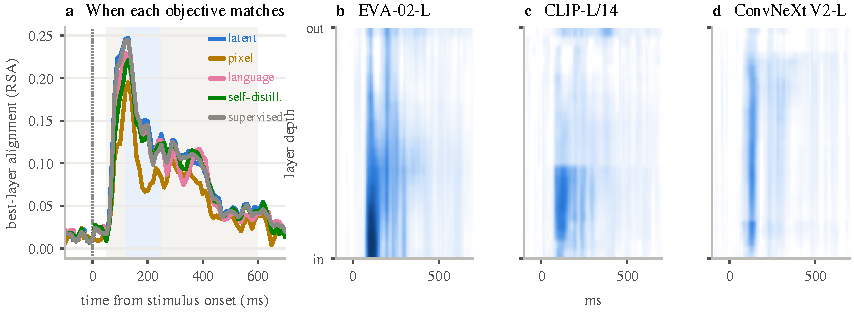
\includegraphics[width=\linewidth]{figures/time.pdf}
  \caption{\textbf{When networks match the brain.} \textbf{a}~Best-layer alignment (RSA) over
    time, median over the models of each objective class. Shaded: early, semantic and late
    windows. \textbf{b--d}~Layer$\times$time alignment for the best-aligned model (EVA-02-L), a
    typical one (CLIP-L/14) and one of the worst (ConvNeXt~V2-L, masked autoencoding); common
    colour scale.}
  \label{fig:time}
\end{figure}

\begin{figure}[t]
  \centering
  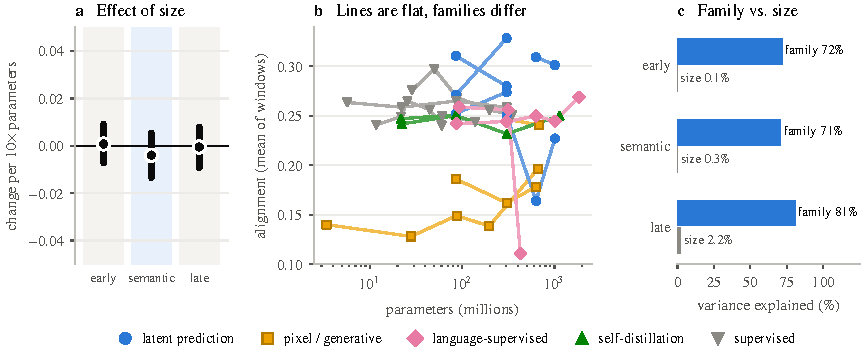
\includegraphics[width=\linewidth]{figures/scale.pdf}
  \caption{\textbf{Size does not move alignment; the model family does.} \textbf{a}~Within-family
    change in alignment per tenfold increase in parameters, with 95\% intervals.
    \textbf{b}~Alignment (mean of the three windows) against size for all \vNall{} models; lines
    join members of a family. \textbf{c}~Share of the variance between models explained by model
    family and by size within family. Per-window panels are in \cref{fig:scalewin}.}
  \label{fig:scale}
\end{figure}

% =====================================================================
\section{Theory: spectral trajectories}
\label{sec:theory}

\paragraph{Setting.} Inputs $x\in\R^d$ have $\E x = 0$ and $\Cov(x) = \Sigma$. A depth-$T$ linear
network computes $h_t = W_{t:1}x$ with $W_{t:1} = W_t\cdots W_1$, trained on
\begin{equation}
  J(W_1,\dots,W_T) = \E\lVert Mx - W_{T:1}x\rVert^2 + \lambda\textstyle\sum_t \fro{W_t}^2 ,
  \label{eq:objective}
\end{equation}
where $M$ encodes the objective: a task map for supervised learning, $I$ for pixel
reconstruction, or a normalized embedding for latent prediction. The variance structure of
layer $t$ is its \emph{whitened Gram} $\tilde G_t = \Sigma^{1/2} W_{t:1}^\T W_{t:1}\Sigma^{1/2}$,
whose eigenvalues are the variances of $h_t$.

\begin{lemma}[CKA is a cosine of whitened Grams]
\label{lem:cka}
For $h = Ax$ and $b = Bx$, population linear CKA equals
$\ip{\tilde G_A}{\tilde G_B}/(\fro{\tilde G_A}\fro{\tilde G_B})$.
\end{lemma}

\begin{proposition}[Spectral matching]
\label{prop:match}
Let $\tilde G_A \propto \Sigma^a$ and $\tilde G_B \propto \Sigma^b$, with $\Sigma$ not a
multiple of the identity. Then $\CKA$ is a unimodal function of $a$ with its unique maximum,
equal to $1$, at $a = b$.
\end{proposition}

\begin{proposition}[Spectral trajectories]
\label{prop:traj}
At every stationary point of \eqref{eq:objective}, the layers are balanced and
$W_{t:1}^\T W_{t:1} = (W_{T:1}^\T W_{T:1})^{t/T}$. If the end-to-end Gram is a function of the
input statistics, $W_{T:1}^\T W_{T:1} = \Sigma^{2c}$ on the retained eigenspaces (which holds
for $M = \Sigma^c$ as $\lambda\to0$), then
\begin{equation}
  \tilde G_t = \Sigma^{\,1 + 2ct/T}, \qquad t = 1,\dots,T .
\end{equation}
The exponent runs linearly from the input's ($1$) to the objective's endpoint ($1 + 2c$).
\end{proposition}

\begin{corollary}[Objective, not scale]
\label{cor:scale}
Width does not enter \cref{prop:traj}, and depth changes only the grid $\{t/T\}$ on a fixed
path. By \cref{prop:match}, the stages a network can match are those whose exponents lie on its
path: pixel reconstruction ($c=0$) stays at the input spectrum at every layer, while a whitened
latent target ($c=-\tfrac12$) sweeps the whole range $[0,1]$.
\end{corollary}

\noindent
Proofs are in \cref{app:proofs}. \Cref{fig:spectral}a confirms \cref{prop:traj} by gradient
descent: layer exponents fall exactly on $1-t/T$ for a latent target and stay at $1$ for
reconstruction, for every width and depth tested. Real networks behave as the theory predicts
in the way the theory describes (\cref{fig:depth}a). Every class of objective starts near the
input's spectrum in its first layers and descends with depth, as \cref{prop:traj} requires; the
endpoint depends on the objective, highest for pixel and generative objectives, which return to
the input's spectrum at the output, and lowest for self-distillation. Low-level content peaks in
the middle of the network and is weakest throughout for pixel objectives
(\cref{fig:depth}b); semantic content rises toward the output for supervised and
language-supervised networks (\cref{fig:depth}c).

\begin{figure}[t]
  \centering
  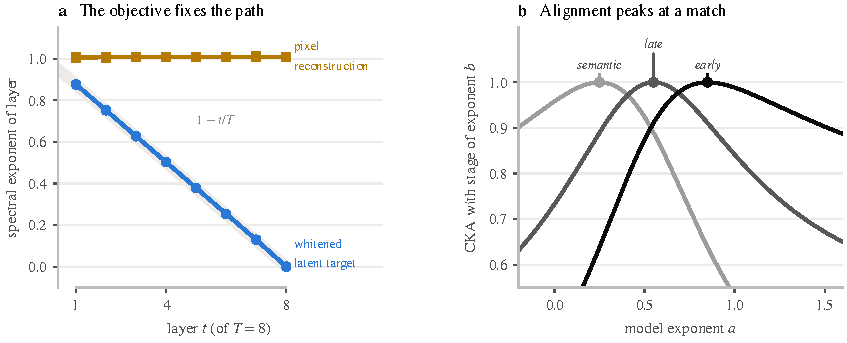
\includegraphics[width=0.86\linewidth]{figures/theory2.pdf}
  \caption{\textbf{Spectral trajectories in theory.} \textbf{a}~Deep linear networks under a
    natural-image spectrum (eigenvalues $\propto k^{-1}$): the exponent of each layer's whitened
    Gram, for pixel reconstruction and a whitened latent target (\cref{prop:traj}).
    \textbf{b}~CKA between spectra $\Sigma^a$ and $\Sigma^b$ peaks at $a=b$ (\cref{prop:match});
    $b$ is set to the value fitted for each EEG window in \cref{sec:law}.}
  \label{fig:spectral}
\end{figure}

\begin{figure}[t]
  \centering
  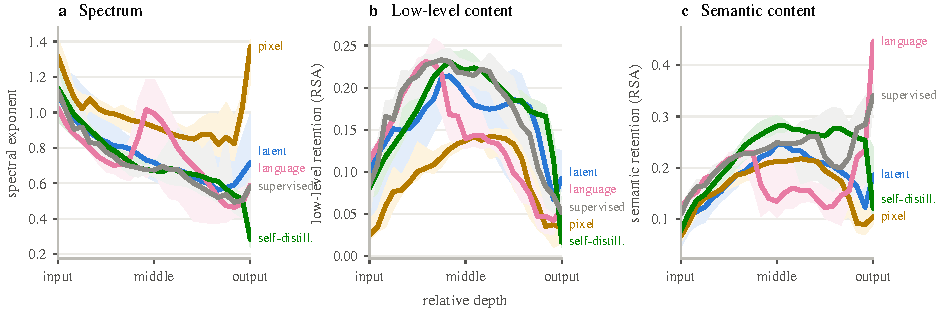
\includegraphics[width=\linewidth]{figures/depth.pdf}
  \caption{\textbf{What real networks do through depth}, measured without neural data. Median
    (line) and interquartile range (shade) over the models of each objective class, against
    relative depth. \textbf{a}~Spectral exponent. \textbf{b}~Low-level content (RSA with a
    Gabor-energy model). \textbf{c}~Semantic content (RSA with human category labels).}
  \label{fig:depth}
\end{figure}

% =====================================================================
\section{A brain-free law}
\label{sec:law}

\paragraph{Proxies.} For every layer we compute three quantities from the model alone, on the
same 200 images: the spectral exponent $\alpha(\ell)$, the power-law decay of the eigenvalues
of the centred Gram (ranks 2--50); low-level retention $L(\ell)$, RSA with a Gabor-energy model
of the images (4 scales, 8 orientations); and semantic retention $S(\ell)$, RSA with human
category labels from THINGSplus~\citep{hebart2023things} (53 categories).

\paragraph{Law.} Guided by \cref{prop:match}, the score in window $w$ is
\begin{equation}
  \widehat{\text{score}}_w = c_0 + c_1 L_{\max} + c_2 S_{\max} - c_3\, m_w^2, \qquad
  m_w = \min_\ell \lvert \alpha(\ell) - b_w \rvert ,
  \label{eq:law}
\end{equation}
where $b_w$ is the window's preferred exponent. We fit $b_w$ by leave-one-family-out
cross-validation on a fixed grid and $c$ by least squares, on \vNdev{} development models.

\paragraph{Fit.} Predicting each family from a law fit on the others gives Spearman
$\rho$ = \vCvEarly, \vCvMid{} and \vCvLate{} (early, semantic, late; $R^2$ = \vCvREarly,
\vCvRMid{} and \vCvRLate). The fitted exponents are $b$ = \vBEarly, \vBMid{} and \vBLate: the
early window prefers spectra close to the input's, the semantic window the flattest, and the
late window lies between (\cref{fig:spectral}b; measured exponents of every model in
\cref{fig:measured}). Nothing in the fitting procedure imposes
this ordering.

% =====================================================================
\section{Held-out test}
\label{sec:heldout}

\paragraph{Protocol.} We chose \vNheld{} models that had never been analysed, spanning seven
objectives: DINO~\citep{caron2021dino}, ConvNeXt~V2 with fully convolutional masked
autoencoding~\citep{woo2023convnextv2}, EVA-02~\citep{fang2024eva02}, SigLIP~\citep{zhai2023siglip},
AIMv2~\citep{fini2025aimv2}, data2vec~\citep{baevski2022data2vec} and
BEiT~\citep{bao2022beit}. We extracted their features, computed their proxies, and wrote the
frozen law's predictions to a file whose SHA-256 (\vHash\ldots) was published in the public
repository before their alignment with the brain was computed. The analysis code refuses to
score held-out models unless that file matches its hash.

\paragraph{Decision rule (registered).} The law is supported if the lower 95\% bound of the
Spearman correlation between predicted and observed scores is positive in both the early and
the late window, and the law's correlation exceeds that of a log-parameters baseline in both. The
bootstrap resamples subjects, stimuli \emph{and models}, so the interval reflects the number of
held-out models.

\paragraph{Result.} The verdict is \textbf{\vLawVerdict} (\cref{fig:law}). The law's correlations
are \vRhoEarly{} (early), \vRhoMid{} (semantic) and \vRhoLate{} (late). Size gives \vParEarly,
\vParMid{} and \vParLate. EVA-02-L, the best-aligned of all \vNall{} models in the early window,
was among the law's four highest predictions; all five masked-autoencoding ConvNeXt~V2 models were
predicted to be, and are, among the six worst-aligned held-out models in every window
(\cref{tab:heldout}).

\begin{figure}[t]
  \centering
  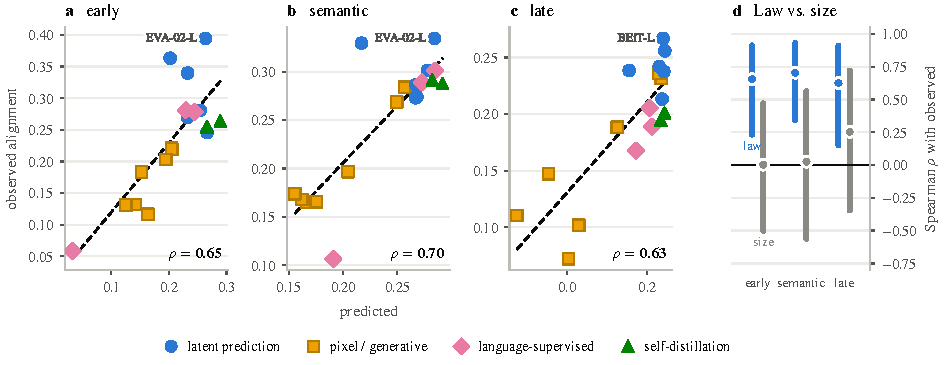
\includegraphics[width=\linewidth]{figures/law.pdf}
  \caption{\textbf{The registered law predicts unseen models.} \textbf{a--c}~Predicted against
    observed alignment for the \vNheld{} held-out models in each window; dashed: least-squares
    line. \textbf{d}~Spearman correlation with the observed scores for the law and for model size,
    with 95\% intervals over subjects, stimuli and models. Development models are shown in
    \cref{fig:lawfull}.}
  \label{fig:law}
\end{figure}

\begin{table}[t]
\centering\small
\caption{\textbf{Held-out models}: registered predictions and observed noise-ceiling-normalized
  window scores.}
\label{tab:heldout}
\begin{tabular}{@{}llrcccccc@{}}
\toprule
 & & & \multicolumn{2}{c}{early} & \multicolumn{2}{c}{semantic} & \multicolumn{2}{c}{late} \\
\cmidrule(lr){4-5}\cmidrule(lr){6-7}\cmidrule(l){8-9}
Model & Objective class & Params (M) & pred. & obs. & pred. & obs. & pred. & obs. \\
\midrule
\ifhrhvtwo\tabinput{generated/tab_heldout.tex}\fi
\bottomrule
\end{tabular}
\end{table}

\paragraph{What carries the law (exploratory).} Three analyses were run after the registered test
(\cref{fig:ablation}). First, low-level retention alone predicts the held-out models almost as
well as the full law; the spectral term adds most in the late window, where it is needed to fit the
development models. Second, the early-window result depends on the ConvNeXt~V2 family: without it,
the correlation falls to \vNoFcEarly{}, while the semantic (\vNoFcMid) and late (\vNoFcLate)
correlations are less affected. Third, the paired difference between the law and the size
baseline has intervals that touch zero; the law outperforms size clearly in point estimate but not
decisively.

\begin{figure}[t]
  \centering
  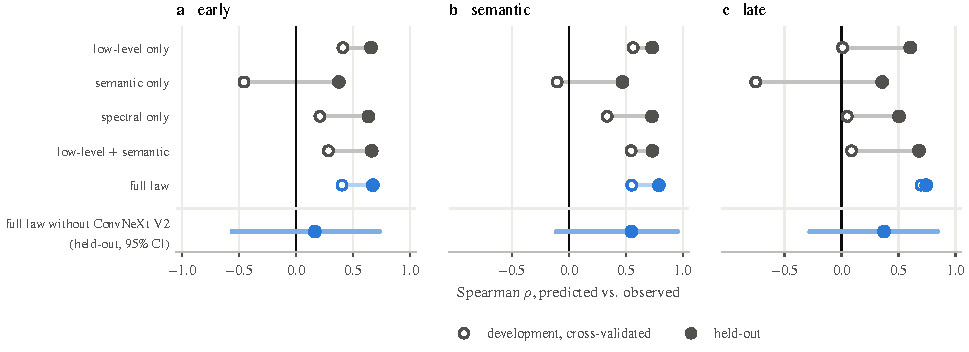
\includegraphics[width=\linewidth]{figures/ablation.pdf}
  \caption{\textbf{Which components carry the law} (exploratory). Spearman correlation for laws
    restricted to subsets of the proxies, cross-validated on development models (hollow) and on the
    held-out models (filled). Bottom: the registered law on held-out models without the ConvNeXt~V2
    family (95\% interval over models).}
  \label{fig:ablation}
\end{figure}

% =====================================================================
\ifhrhconv
\section{Convergence between models}
\label{sec:convergence}

\paragraph{Design.} PRH is a claim about models converging with each other, so we also measure
that directly, with its own metric: mutual nearest neighbours ($k=10$) between every pair of the
\vNall{} models, at four relative depths. A model's agreement at a depth is its mean over models
of other families. Before running the analysis we pre-specified two predictions: (P1) agreement
at the readout rises with size within families, as PRH reports; (P2) that rise is larger at the
readout than at mid depth. Intervals come from 100 subsamples of 80\% of the stimuli and are
approximate, because nearest-neighbour agreement depends on the number of stimuli.

\paragraph{Both predictions failed.} The within-family slope at the readout is \vConvSlopeOut{}
per decade; scale adds agreement mainly at mid depth (\vConvSlopeMid; \cref{fig:convergence}a).

\paragraph{Models diverge with depth, and objectives decide where they end.} Agreement between
models falls from \vAgreeQ{} at a quarter of the depth to \vAgreeOut{} at the readout. Between
models with different objectives it falls throughout (\vAgreeDiffQ{} to \vAgreeDiffOut), while
models with the same objective, after diverging, re-converge at the readout (\vAgreeSameTQ{} to
\vAgreeSameOut; \cref{fig:convergence}b). This is the picture of \cref{prop:traj}: a common
start at the input's statistics and paths that separate toward objective-specific endpoints.

\paragraph{Agreement and the brain.} Models that agree more with others at the readout are also
better aligned with the brain in the early (Spearman $\rho$ = \vConvBrainEarly) and semantic
(\vConvBrainMid) windows, but not the late window (\vConvBrainLate; \cref{fig:convergence}c).
Agreement between models thus tracks alignment with the first two stages of visual processing,
in line with the PRH intuition, but not with the later stage.

\begin{figure}[t]
  \centering
  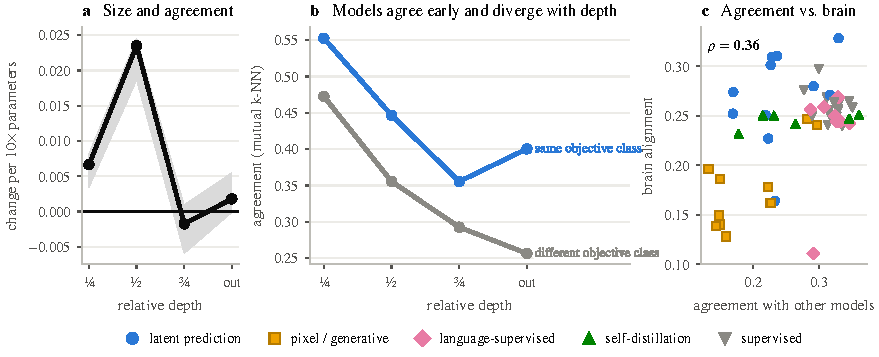
\includegraphics[width=\linewidth]{figures/convergence.pdf}
  \caption{\textbf{Convergence between models} (mutual $k$-NN, the PRH metric). \textbf{a}~Within-family
    change in a model's agreement with other families per tenfold increase in size, by depth (shade:
    approximate 95\% interval). \textbf{b}~Mean agreement between pairs of models with the same or a
    different objective class. \textbf{c}~Readout agreement against brain alignment (mean of the three
    windows).}
  \label{fig:convergence}
\end{figure}
\fi

% =====================================================================
\FloatBarrier
\section{Discussion}
\label{sec:discussion}

\paragraph{What this means for convergence.} Across six families and more than two orders of
magnitude, size leaves alignment with every stage of visual processing where it is, and it adds
little agreement between models at the readout. What moves it is the objective, through the spectra it imposes on the
layers. In the Heraclitean picture, a network does not approach a fixed Form; it follows a path
laid out by what it learns to predict, and matches the moments of perception that lie on that
path.

\paragraph{Predictions that failed.} Earlier in this project we pre-specified, in code and before the
analysis, two predictions that did not survive. We expected scale to raise alignment in the semantic window; it did not. We expected
objectives with dense readouts, as a class, to exceed single-readout networks in the early and late
windows; the pooled test was not supported, because masked autoencoders fell below their references
while I-JEPA rose above them, and a pre-specified replication with
V-JEPA~2~\citep{assran2025vjepa2} also failed. The spectral account was developed in response, and the held-out test above is its
first prospective evaluation. Two further pre-specified predictions, about where scale adds
agreement between models, failed as well (\cref{sec:convergence}).

\paragraph{Limitations.} The theory is linear. EEG has coarse spatial resolution; the analysis
should be repeated with MEG and fMRI and with the THINGS training images. The held-out set is
\vNheld{} models, and the early-window result leans on one family. The law was fit on \vNdev{}
development models: the three V-JEPA~2 models were not part of the fit, because their scores were
missing from the development summary at the time. Size matching across objectives is approximate.

\paragraph{Reproducibility.} Every number and figure is produced from public data and weights by
the released pipeline; numbers in the text are generated, not typed. The registered predictions and
their hash are in the repository.

{\small
\bibliographystyle{abbrvnat}
\bibliography{refs}
}

% =====================================================================
\clearpage
\appendix
\section{Proofs}
\label{app:proofs}

Throughout, $W_{t:s} = W_t\cdots W_s$ and $W_{s-1:s} = I$.

\paragraph{Proof of \cref{lem:cka}.} $\Cov(h,b) = A\Sigma B^\T$, so
$\fro{\Cov(h,b)}^2 = \operatorname{tr}(B\Sigma A^\T A\Sigma B^\T)
= \operatorname{tr}(\tilde G_A\tilde G_B)$ with $\tilde G_A = \Sigma^{1/2}A^\T A\Sigma^{1/2}$.
Likewise $\fro{\Cov(h)} = \fro{A\Sigma A^\T} = \fro{\tilde G_A}$, because $A\Sigma A^\T$ and
$\tilde G_A$ share their nonzero eigenvalues. Substituting into
$\CKA = \fro{\Cov(h,b)}^2/(\fro{\Cov(h)}\fro{\Cov(b)})$ gives the claim. \qed

\paragraph{Proof of \cref{prop:match}.} Let $\lambda_i>0$ be the eigenvalues of $\Sigma$. By
\cref{lem:cka}, $\CKA = \sum_i \lambda_i^{a+b} / (\sum_i\lambda_i^{2a}\sum_i\lambda_i^{2b})^{1/2}$,
which is at most $1$ by Cauchy--Schwarz, with equality iff $\lambda^a\propto\lambda^b$, that is,
iff $a=b$ when the $\lambda_i$ are not all equal. For unimodality write
$f(a) = \log\sum_i\lambda_i^{a+b} - \tfrac12\log\sum_i\lambda_i^{2a} + \text{const}$ and let
$g(c) = \E_{p_c}[\log\lambda]$ with $p_c(i)\propto\lambda_i^c$. Then
$f'(a) = g(a+b) - g(2a)$, and $g'(c) = \operatorname{Var}_{p_c}(\log\lambda) > 0$, so $g$ is
strictly increasing and $f'(a)>0$ iff $a+b>2a$, that is, iff $a<b$. \qed

\paragraph{Proof of \cref{prop:traj}.} Write $\ell(P) = \E\lVert Mx-Px\rVert^2$ with
$\Gamma = \nabla\ell$. Then $\nabla_{W_t}\ell = W_{T:t+1}^\T\Gamma W_{t-1:1}^\T$, hence
$W_{t+1}^\T\nabla_{W_{t+1}}\ell = (\nabla_{W_t}\ell)W_t^\T$ for any differentiable $\ell$.
Stationarity gives $\nabla_{W_t}\ell = -2\lambda W_t$, so $W_{t+1}^\T W_{t+1} = W_tW_t^\T$
(balancedness). As in the isotropic case, induction on $t$ gives
$W_{t:1}^\T(W_tW_t^\T)^jW_{t:1} = (W_1^\T W_1)^{t+j}$; with $j=0$, $W_{t:1}^\T W_{t:1} =
(W_1^\T W_1)^t = (W_{T:1}^\T W_{T:1})^{t/T}$, using the unique PSD root. If
$W_{T:1}^\T W_{T:1} = \Sigma^{2c}$, it commutes with $\Sigma$, so
$\tilde G_t = \Sigma^{1/2}\Sigma^{2ct/T}\Sigma^{1/2} = \Sigma^{1+2ct/T}$. For $M=\Sigma^c$, the
minimizer of $\ell$ is $P=M$; as $\lambda\to0$, stationary end-to-end maps converge to $M$ on the
eigenspaces they retain, which gives the stated form there. \qed

\section{Implementation details}
\label{app:impl}

\paragraph{Reliable bins.} With $\mu_0,\sigma_0$ the mean and standard deviation of split-half
reliability over pre-stimulus bins, a post-onset bin is significant if
$r_t > \mu_0 + z_{1-\alpha/m}\sigma_0$ ($m$ post-onset bins, $\alpha=0.05$); only runs of at
least three significant bins are kept. Reliable bins span about 70--470\,ms in every subject.

\paragraph{Proxies.} Gram matrices are double-centred before the eigendecomposition. The Gabor
model uses complex filters with one-octave bandwidth at wavelengths of 4, 8, 16 and 32 pixels on
$128\times128$ grayscale images, energy pooled on a $4\times4$ grid and log-compressed. The
semantic kernel is the Jaccard distance between THINGSplus category sets; six images without a
category are excluded from that kernel only.

\paragraph{Law and baselines.} $b_w\in\{0, 0.05, \dots, 3\}$; ridge $10^{-6}$. The size baseline
is a least-squares fit of window score on $\log_{10}$ parameters on the same development models.



\section{Additional figures}
\label{app:figs}

\begin{figure}[h]
  \centering
  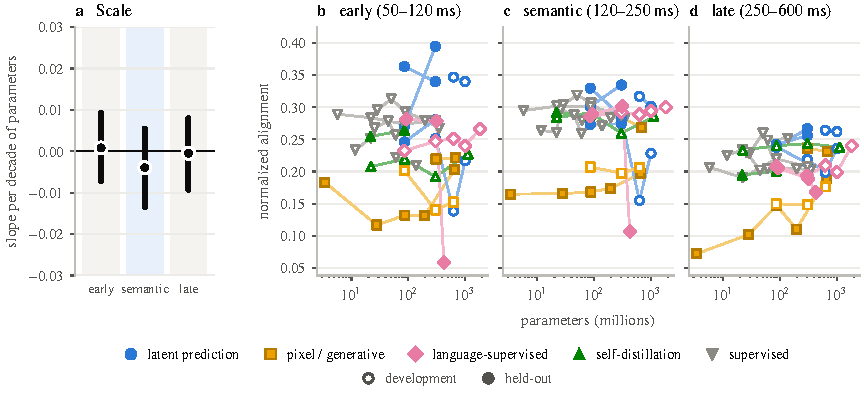
\includegraphics[width=\linewidth]{figures/scale_windows.pdf}
  \caption{\textbf{Scale, window by window.} \textbf{a}~Within-family slopes. \textbf{b--d}~Window
    score against size for every model; hollow: development, filled: held-out.}
  \label{fig:scalewin}
\end{figure}

\begin{figure}[h]
  \centering
  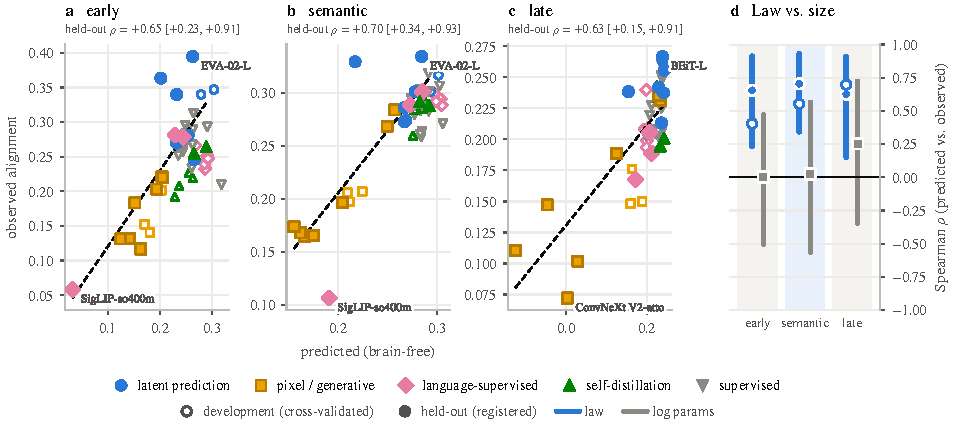
\includegraphics[width=\linewidth]{figures/law_full.pdf}
  \caption{\textbf{Law, development and held-out.} Hollow: development models, each predicted by
    a law fit without its family. Filled: held-out models (registered predictions). \textbf{d}~Held-out
    correlations with 95\% intervals (filled) and cross-validated development correlations
    (hollow).}
  \label{fig:lawfull}
\end{figure}

\begin{figure}[h]
  \centering
  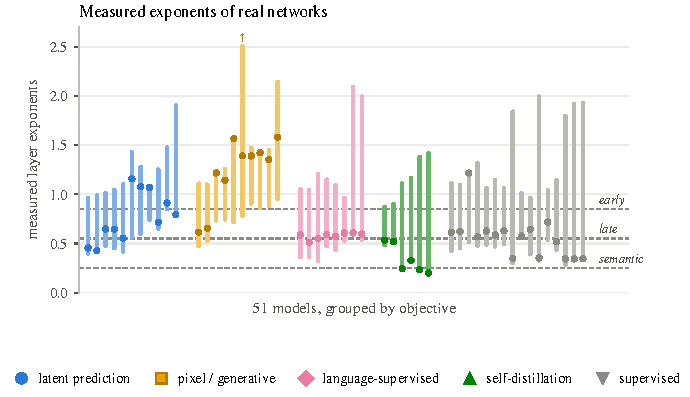
\includegraphics[width=\linewidth]{figures/spectral_measured.pdf}
  \caption{\textbf{Measured exponents of every model}: range across layers (bar) and final layer
    (dot), grouped by objective; dashed lines mark the windows' fitted exponents.}
  \label{fig:measured}
\end{figure}

\begin{figure}[h]
  \centering
  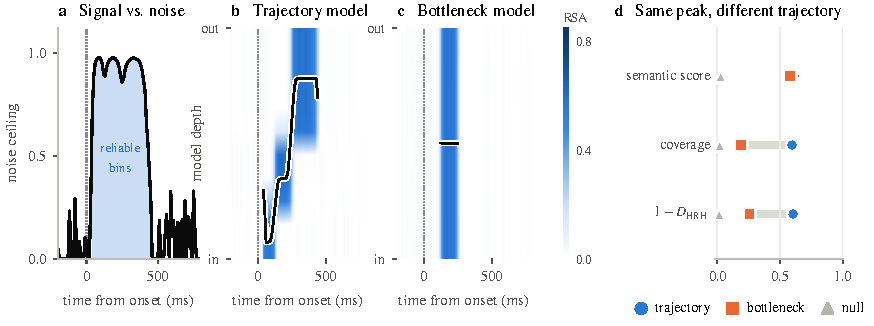
\includegraphics[width=\linewidth]{figures/validation.pdf}
  \caption{\textbf{Validation on synthetic ground truth.} Simulated EEG with three planted
    regimes. \textbf{a}~The per-bin ceiling and the reliable-bin test recover the signal span.
    \textbf{b,c}~Layer$\times$time alignment of a model whose layers walk through the regimes and
    of a model that matches one regime only. \textbf{d}~Temporal coverage separates them.}
  \label{fig:validation}
\end{figure}

\end{document}
